% ОБЯЗАТЕЛЬНО ИМЕННО ТАКОЙ documentclass!
% (Основной кегль = 14pt, поэтому необходим extsizes)
% Формат, разумеется, А4
% article потому что стандарт не подразумевает разделов
% Глава = section, Параграф = subsection
% (понятия "глава" и "параграф" из стандарта)
\documentclass[a4paper,article,14pt]{extarticle}

% Подключаем главный пакет со всем необходимым
\usepackage{spbudiploma}

% Пакеты по желанию (самые распространенные)
% Хитрые мат. символы
\usepackage{euscript}
% Таблицы
\usepackage{longtable}
\usepackage{makecell}
% Картинки (можно встявлять даже pdf)
\usepackage[pdftex]{graphicx}

\usepackage{amsthm,amssymb, amsmath}
\usepackage{textcomp}
\usepackage{amsmath}
\usepackage{comment}
\usepackage{svg}


\begin{document}

% Титульник в файле titlepage.tex
% --------------------- Стандарт СПбГУ для ВКР --------------------------
% Автор: Тоскин Николай, itonik@me.com
% Если заметили ошибку, напишите на email
% Если хотите добавить изменение самостоятельно, GitHub: . PR-s welcome!
% Использованы материалы:
% habr.com/ru/post/144648/
% cpsconf.ru
% Текст:
% http://edu.spbu.ru/images/data/normativ_acts/local/20181030_10432_1.pdf
% Титульный лист:
% http://edu.spbu.ru/images/data/normativ_acts/local/20180703_6616_1.pdf
% -----------------------------------------------------------------------

% Титульный лист диплома СПбГУ
% Временное удаление foot на titlepage
\newgeometry{left=30mm, top=20mm, right=15mm, bottom=20mm, nohead, nofoot}
\begin{titlepage}
\begin{center}
% Первый символ съедается, первым знаком поставлен Ы
\textbf{Санкт--Петербургский}
\textbf{государственный университет}

\vspace{35mm}

\textbf{\textit{\large Ковалев Святослав Сергеевич}} \\[8mm]
% Название
\textbf{\large Выпускная квалификационная работа}\\[3mm]
\textbf{\textit{\large Прогнозирование временных рядов методами машинного обучения}}

\vspace{20mm}
% TODO: Узнать как правильно
Уровень образования: бакалавриат\\
Направление 01.03.02 «Прикладная математика и информатика»\\
«Прикладная математика, фундаментальная информатика и программирование»\\


% Научный руководитель, рецензент
% Сходить в уч отдел и узнать, правильно ли
\begin{flushright}
{Научный руководитель:} \\
% TODO: Узнать кафедру
профессор, кафедра компьютерных технологий \\ и систем, д.ф. - м.н.  Буре~Владимир Мансурович
\end{flushright}
\begin{flushright}
{Рецензент:} \\
% TODO: Узнать кафедру
профессор, кафедра компьютерных технологий \\и систем, д.ф. - м.н.  Буре~Владимир Мансурович
\end{flushright}

\vfill 

{Санкт-Петербург}
\par{2020 г.}
\end{center}
\end{titlepage}
% Возвращаем настройки geometry обратно (то, что объявлено в преамбуле)
\restoregeometry
% Добавляем 1 к счетчику страниц ПОСЛЕ titlepage, чтобы исключить 
% влияние titlepage environment
\addtocounter{page}{1}

% Содержание
\tableofcontents
\pagebreak

\specialsection{Введение}

Прогнозирование временных рядов - одна из главных задач в экономике и финансах.
Хотя эта задача достаточно изучена для определенного класса временных рядов, остаются нерешенные проблемы.
Например, прогнозирование цен биржевых торгов.
\par
Прогнозирование биржевых цен позволяет крупным компаниям принимать стратегические решения, а частным трейдерам совершать выгодные сделки.
Цель этой работы - показать эффективность алгоритмов машинного обучения в вопросе прогнозирования цен биржевых торгов.
Чтобы показать эффективность алгоритмов, были использованы исторические данные, предоставляемые Yahoo Finance ~\cite{yahoo}, по нескольким финансовым инструментам.

\specialsection{Постановка задачи}

Даны временные ряды
\begin{equation}
    {X_{i} = \{x_{i,t}, t=\overline{1,k}\},\quad i=\overline{1,m}},\label{eq:equation}
\end{equation}
где $m$~--- общее количество рядов, а размер всех рядов совпадает и равен $k$.
Цель~--- предсказать значение всех рядов с лагом $n$.
Для этого требуется построить такую модель $A(X_i)$, что
\begin{equation}
    A(X_i)=x_{i, k+n}.\label{eq:equation2}
\end{equation}


\section{Обзор методов}

Для предсказания временных рядов использовались модели ARIMA (Autoregressive Integrated Moving Averate), VAR (Vector Autoregressive model), Wavelet, Fourier Extrapolation и Stacking.
Каждая из моделей сравнивалась с "наивной" моделью, которая предсказывала последнее известное значение на весь горизонт прогнозирования.

\par
Ниже приводится краткий обзор моделей:

1.
ARIMA~\cite{arima} - Модель ARIMA является классическим методом эконометрики для прогнозирования временных рядов.
Применение ARIMA для прогнозирования биржевых цен уже рассматривалось ранее~\cite{my_arima_article}.

\textbf{TODO: написать формулы.}

2.
VAR~\cite{var} - Модель VAR позволяет находить линейные зависимости между компонентами многомерных временных рядов.

\textbf{TODO: написать формулы}

3.
Wavelet~\cite{wavelet} - В основе модели лежит дискретное вейвлет преобразование.
Исходный ряд раскладывается на $k$ рядов, каждый из которых предсказывается по отдельности при помощи ARIMA, после чего выполняется обратное преобразование.
Использовалась реализация вейвлет функций из пакета PyWavelets~\cite{pywt}.
В качестве вейвлет-функций используются койфлеты, так как показали наилучший результат.

4.
Fourier Extrapolation - модель экстраполяции фурье.
Часто используется при обработке сигналов и может быть применена для работы с финансовыми временными рядами.
\textbf{TODO: написать формулы}

5.
Baseline - "наивная" модель, которая предсказывает последнее известное значение на весь горизонт прогнозирования.

6.
Stacking - ансамблевая модель, основанная на градиентном бустинге над решениями, описанными выше.
Обычно комбинация решений и создание ансамблей улучшает качество моделей.
\textbf{TODO: написать формулы}

\section{Оценка качества моделей}

Оценка качества моделей производилась методом кросс-валидации для временных рядов:

1.
Выборка делится на тренировочную и тестовую.

2.
Исходные ряды прогнозируются на $n$ точек вперед.

3.
Считаем целевую метрику, сравнивая предсказание с фактическими ценами и сохраняем.

4.
Первая точка из тестовой выборки перемещается в тренировочную

5.
Повторяем п. 2 - п. 4 до тех пор, пока в тестовой выборке будет оставаться больше $n$ точек.

6.
Посчитать средневзвешенное значение для всего полученного массива метрик.

В предложенном алгоритме стоит пояснить п. 3.
Можно считать близость двух векторов (вектор предсказаний и вектор фактических цен), либо можно считать близость предсказания в последней точке прогноза.
В первом случае мы оценим модель на то, насколько точно она прогнозирует общую картину изменения цен (скачки цен внутри периода), при этом мы пренебрегаем тем, что цена в конце периода может быть важнее, чем остальные цены.
Во втором случае мы оценим насколько точно модель прогнозирует цену по заданному горизонту, игнорируя общую картину.
Есть третий подход, который является компромисом.
Можно для каждого дня прогноза оценивать близость с фактической ценой в этот день.
Тогда для каждого прогнозного дня будет свое значение метрики.

В этой работе будем использовать второй и третий подход, так как их проще интерпретировать.

В качестве метрики будем использовать: Mean absolute error (MAE), mean absolute percentage error (MAPE), root mean squared error (RMSE).

\section{Воспроизводимость вычислений}

Для того, чтобы полученные результаты были достоверными и воспроизводимыми, а также чтобы полученные модели можно было использовать как фреймворк для произвольных данных в будущем, был построен конвейер (pipeline) для обработки данных.
Для реализации конвейера использовался инструмент snakemake~\cite{snakemake}.
Snakemake позволяет определять "правила" (rules) для обработки данных.
Каждое правило может иметь входные и выходные файлы.
Правило должно генерировать из входного файла выходной.
Если входной файл не существует, то ищется другое правило, которое генерирует этот файл.
Таким образом, получается ациклический граф работ, при помощи которого snakemake планирует и исполняет все необходимые работы для того, чтобы получить результат.

Решения задачи использовался граф работ, изображенный на рис.~\ref{graph_dag}.
\begin{figure}[ht]
\begin{center}
\scalebox{0.4}{
   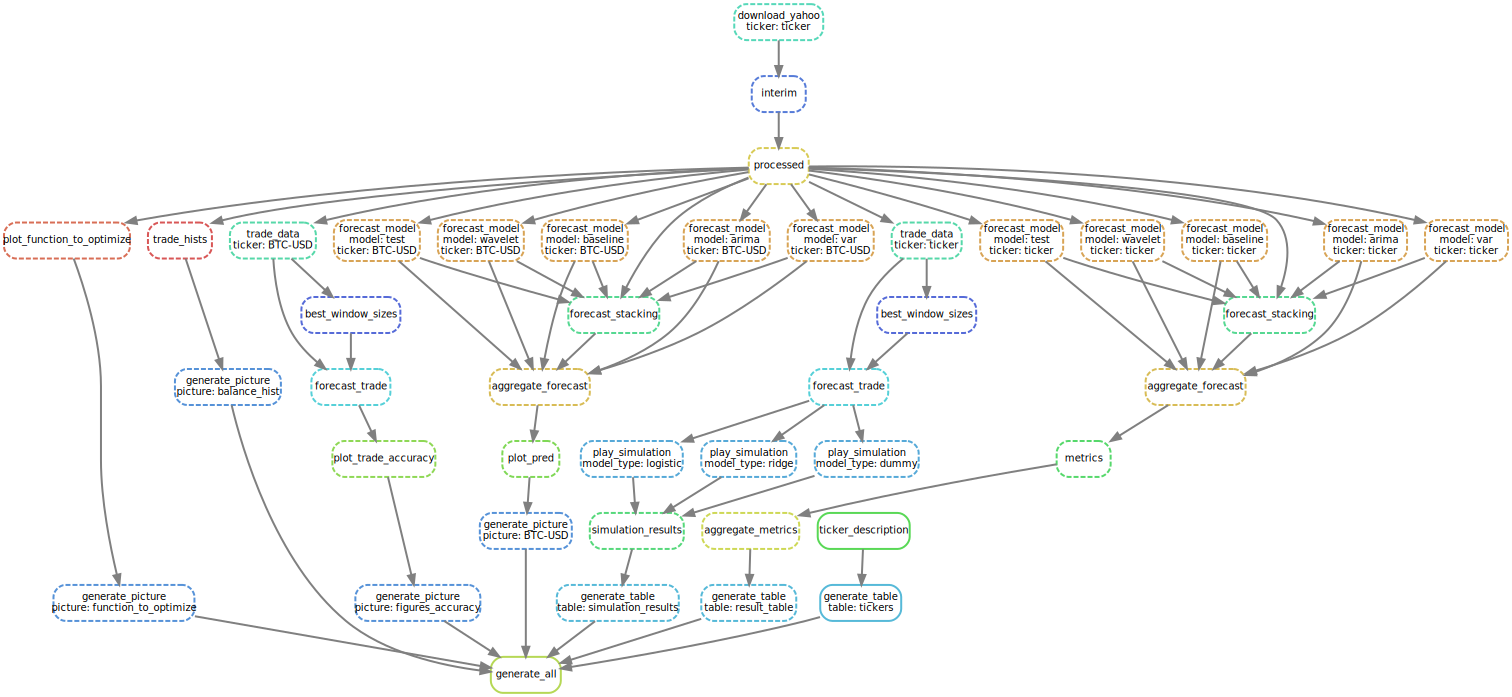
\includegraphics{../dag.svg}
}
\caption{
\label{graph_dag}
     Ациклический граф работ.}
\end {center}
\end {figure}
Шаги, исполняемые конвейером:

1.
Загружаем данные

2.
Преобразуем исходные данные в удобный формат.

3.
Используем модели для построения прогнозов по заданным датам и генерации тестовой выборки.

4.
Полученные данные используются для генерации графиков и подсчета метрик.

5.
Генерируем код LaTeX для вставки графиков и таблиц с результатами

\section{Эксперимент}

Были взяты данные с Yahoo Finance~\cite{yahoo}.

\input{../reports/tickers.tex}


Для каждого временного ряда применялась каждая из моделей.
Модель VAR применялась сразу для всех временных рядов.
Сравнение результатов происходило по метрикам:

MAE (Mean absolute error):
\begin{equation}
    MAE = \sum_{i=1}^{n} \frac{|y_i - x_i|}{n}\label{eq:mae}
\end{equation}

MAPE (Mean absolute percentage error):

\begin{equation}
    MAPE = \frac{1}{n} \sum_{i=1}^{n} \left| \frac{y_i - x_i}{y_i} \right|\label{eq:mape}
\end{equation}

\begin{comment}
RMSE (Root mean square error)
\begin{equation}
    RMSE = \sqrt{\sum_{i=1}^{n} \frac{(x_i - y_i) ^ 2}{n}}\label{eq:rmse}
\end{equation}
\end{comment}

Результаты можно наблюдать в таблице~\ref{result_table}.
\input{../reports/result_table.tex}

Также результат прогноза можно видеть  на рис.~\ref{graph0}.
\documentclass[12pt]{article}
\begin{document}
Hello world!
$Hello world!$ %math mode
\end{document}

\section{Моделирование торговли на бирже}
\subsection{Постановка задачи}

Помимо классической задачи прогонозирования временных рядов может быть полезно использовать альтернативный подход.
Будем моделировать торговлю на бирже.
Пусть в нулевой момент имеется $C$ долларов, на которые можно купить другой актив по цене $price_i$ в момент времени $i$.
Торговля продолжается на протяжении определенного периода (неделя, месяц, год), в конце которого все активы продаются по текущей цене.
Задача - максимизировать итоговое количество долларов.
Также для удобства будем пользоваться следующей формулой:
$$profit = \frac{revenue - cost}{cost} * 100$$

Сведем задачу к задаче классификации.
Каждую точку исходного временного ряд разметим на три класса: "sell", "buy", "hold":

sell - означает, что скоро цена значительно снизится, а следовательно нужно продавать активы;
buy - означает, что скоро цена значительно повысится, а следовательно нужно покупать активы;
hold - означает, что цена в ближайшее время значительно не изменится, а значит ничего делать не нужно.

Выберем горизонт прогнозирования $n$ и сформируем обучающую выборку.
Для каждой точки посчитаем изменение цены в процентах в момент $i$:
$$dp_i = \frac{price_{i + n} - price_{i}}{price_{i}} * 100$$

Выберем порог $t$, начиная с которого будем считать, что изменение цены значительное и выберем класс для каждой точки по следующему правилу:

\begin{equation}
class_i =
 \begin{cases}
     sell &\text{if $dp_i < -t$}
     \\
     buy &\text{if $dp_i > t$}
     \\
     hold &\text{if $|dp_i| < t$}
 \end{cases}\label{eq:equation3}
\end{equation}

Порог $t$ можно выбирать вручную в зависимости от целей трейдера, но на случай, когда необходимо проанализировать большое количество временных рядов, хотелось бы иметь алгоритм автоматического подбора порога $t$.
Для того, чтобы в дальнейшем было проще оценивать результаты задачи классификации, будем исходить из предпосылки, что данные разбиты на равные классы.

Будем решать задачу одномерной оптимизации, в которой $t$ выступает в качестве независимой переменной.

Введем понятие сбалансированности.
Пусть есть выборка из $N$ элементов, каждый из который принадлежит одному из $k \in K$ классов.
Для каждого класса можно посчитать его долю от общего числа элементов:
$$ \{ \frac{n_1}{N}, \frac{n_2}{N}, ... , \frac{n_K}{N} \} $$

Будем называть классы сбалансированными, когда

$$\frac{n_1}{N} \approx \frac{n_2}{N} \approx ... \approx \frac{n_K}{N}$$

В нашем случае имеем 3 класса, соответственно стремимся к тому, чтобы доля каждого класса составляла $\frac{1}{3}$ от общего числа примеров.

Введем функционал качества:
$$J=\sum{(\frac{n_i}{N} - \frac{1}{K}) ^ 2}$$

где $n_i$ - количество элементов, принадлежащих классу $i, i < K$.
Будем считать, что разбиение на классы зависит от порога $t$.
Тогда можем автоматически выбирать $t$ как решение задачи оптимизации:
$$t_{opt} = argmin_t J$$

Полученная оптимизационная задача решается методом нулевого порядка (например, методом золотого сечения).

Однако для целевой функции не была доказана выпуклость, поэтому могут возникнуть случаи, когда в результате оптимизации будет достигнут локальный минимум.
Пример целевой функции приведен на рис.~\ref{graph-optimization}
\input{../reports/function_to_optimize.tex}
Обычно локальный минимум достигается, когда вся обучающая выборка состоит из одного и того же класса, а параметр $t$ либо отрицателен, либо очень большой.
Чтобы избежать таких случаев рекомендуется ставить ограничения на оптимизационную задачу.
Из постановки задачи следует, что параметр $t$ лежит в промежутке $(0, 100)$.
Однако чаще всего разумные значения параметра лежат в промежутке $(0, 50)$.
Наложим эти ограничения на оптимизационную задачу, а также будем оценивать, какое количество классов выделил алгоритм.
Если не был выделен какой-то класс, то будем сужать промежуток вдвое (уменьшая верхнюю границу).
\linebreak
Полученный метод был применем ко всем выбранным временным рядам.
Таким образом, мы получили размеченную выборку и теперь можем решать задачу классификации.

\subsection{Построение моделей классификации}

Поставим задачу обучения с учителем для полученного датасета.
Необходимо построить функцию $f(x)=d, d \in [sell, buy, hold]$, которая на вход получает информацию о временом ряде, а на выходе принимает решение о продаже, покупке или удержании активов.

Задачу классификации можно решать множеством способов, при проведении эксперимента использовались модели случайного леса и логистической регрессии.

Остается открытым вопрос о том, какую информацию об исходном ряде передавать в модель.
Обычно берут окно фиксированной длины $w$ и в качестве входных данных передают последние $w$ значений временного ряда.
Длина окна - гиперпараметр модели, который необходимо подобрать.

При подборе гиперпараметра будем исходить из горизонта прогнозирования $n$.
Будем оценивать качество модели для каждого значение $w \in [n - \frac{n}{2}; n + \frac{n}{2}]$.

Оценивать качество моделей будем при помощи метрики accuracy, используя кросс-валидацию для временных рядов, как это было описано ранее.

Сравнивать качество метрики можно со случайным угадыванием, то есть считаем, что какая-то модель в каждой точке кросс-валидации дала точность 0.33.

Результаты: \textbf{вставить графики}

\subsection{Симуляция биржевых торгов}

Будем считать, что у трейдера есть возможность купить или продать активы в конце торгового дня (ориентируемся на показатель Close).

Модель предсказывает одно из трех значений: sell, buy, hold.
Трейдер действует точно по инструкции:

sell - продать все имеющиеся активы, если они есть;

buy - купить активы на все деньги;

hold - ничего не делать.

Будем считать, что на бирже всегда есть необходимый объем активов и что цена не меняется в зависимости от приобретенных активов.

Так продолжается на протяжении какого-то периода (неделя, месяц или год), а в конце продаются все активы вне зависимости от цены и подсчитывается количество денег.

Чем дольше выбирается период, тем более точно можно оценить качество алгоритма.

Помимо трейдеров, которые торгуют согласно прогнозам алгоритмов, введем еще двух трейдеров, чтобы оценить качество алгоритмов.
Введем трейдера, которому достоверно известна информация о будущем (идеальная модель).
Также введем трейдера, который случайно принимает решение.
Для того, чтобы уменьшить влияние случайности, посчитаем результаты для ста таких трейдеров и усредним их результат ($profit$).

Результаты: \textbf{вставить таблички, а лучше графики}.


\specialsection{Выводы}

//TODO:

генерировать список моделей

точность в зависимости от длины $w$

Таким образом, использованные методы прогнозирования дают прогноз значительно лучше, чем наивное предсказание.
Учитывая высокую волатильность рынков, этот результат является значимым.
Использованные подходы универсальны и их можно применять для предсказания любых других временных рядов, например, в задачах прогнозирования погоды, городских пробок и различных экономических показателей.
Полученные результаты можно улучшить, если преобразовать исходные ряды.

% Библиография в cpsconf стиле
% Аргумент {1} ниже включает переопределенный стиль с выравниванием слева
\begin{thebibliography}{1}
\bibitem{arima} Магнус Я. Р., Катышев П. К., Пересецкий А. А. Эконометрика. Начальный курс.. М.: Дело, 2004. 576 с.
\bibitem{var} Носко В.П. Эконометрика. Введение в регрессионный анализ временных рядов
\bibitem{snakemake} Köster, Johannes and Rahmann, Sven. “Snakemake - A scalable bioinformatics workflow engine”. Bioinformatics 2012.
\bibitem{wavelet} Wang, F.; Yu, Y.; Zhang, Z.; Li, J.; Zhen, Z.; Li, K. Wavelet Decomposition and Convolutional LSTM Networks Based Improved Deep Learning Model for Solar Irradiance Forecasting. Appl. Sci. 2018, 8, 1286.
\bibitem{yahoo} Yahoo Finance [Электронный ресурс] // Yahoo Finance. \url{URL:  https://finance.yahoo.com/} (дата обращения: 20.12.2020).
\bibitem{my_arima_article} Ковалев С.С. Прогнозирование средневзвешенной цены торгов нефтепродуктами на бирже классическими методами анализа временных рядов. // Процессы управления и устойчивость. 2020. №51.
\bibitem{pywt} Gregory R. Lee, Ralf Gommers, Filip Wasilewski, Kai Wohlfahrt, Aaron O’Leary (2019). PyWavelets: A Python package for wavelet analysis. Journal of Open Source Software, 4(36), 1237
\end{thebibliography}
\end{document}